\chapter{Lecture 26 - Introduction to Two-phase Flow}
\label{ch:ch26}
\section{Objectives}
The objectives of this lecture are:
\begin{enumerate}
\item Provide some basic definitions of two-phase flow relevant to nuclear engineering
\item Qualitatively describe two-phase flow regimes
\item Discuss relevance of two-phase flow for hydraulic and thermal phenomena important for nuclear engineers
\end{enumerate}

\section{Introduction and Disclaimer}
\newthought{For the first six years} this course was taught, no material was presented relating to two-phase flows; it was simply relegated to graduate school for any student who might want to specialize in thermal-hydraulics.  During those six years there was an increasing sense that such an attitude is untenable; two-phase flows are an important element in the engineering of pressurized water reactors and two-phase flow phenomena---which play an essential role in understanding concepts such as ``Departure from Nucleate Boiling'' (DNB) and ``Dry-out'' as mechanisms of ``Critical Heat Flux'' (CHF)---have such relevance that I decided they no longer could be ignored completely.  

\newthought{This version} of the notes includes three lectures on two-phase flow and thermal limits, including this lecture.  The treatment is still elementary but advances to the point where (what I think are) essential two-phase phenomena like sub-cooled nucleate boiling and DNB can be treated quantitatively.  At least one correlation to predict DNB will be presented and, perhaps, that is a bare minimum of coverage.  These three lectures are not intended as a rigorous treatment of two-phase thermal-hydraulics as, of course, they could never accomplish such a feat in such a short time period.  Nonetheless it is hoped that this so-called bare minimum suffices as an introduction.


\section{Definitions}
The following terms are needed for our short treatment of two-phase flow:

\begin{itemize}
\item \textbf{Void Fraction:} for two-phase flow in a channel, the void fraction is the fraction of the cross-sectional flow area that is filled with vapor as given in Equation \ref{eq:void-fraction}:
\index{void fraction}
\begin{equation}
\alpha = \frac{A_{v}}{A_{v}+A_{\ell}}
\label{eq:void-fraction}
\end{equation}
where $A_{v}$ is the area with vapor and $A_{\ell}$ is the area with liquid.

\item \textbf{Static quality:} is the same as what, up until now in these lecture notes, we have been calling ``quality''.  In a two-phase flow it is the fraction of the mass of fluid that is in the vapor form as given in Equation \ref{eq:static-quality}:
\index{quality, static}
\begin{equation}
x_{st} = \frac{m_{v}}{m_v + m_{\ell}}
\label{eq:static-quality}
\end{equation}

\item \textbf{Flow quality:} this is similar to static quality but relates to mass flow rate instead; it is the fraction of the mass flow rate at a channel cross section that is vapor.  This is shown in Equation \ref{eq:flow-quality}:
\begin{equation}
x = \frac{\dot{m}_{v}}{\dot{m}_{v} + \dot{m}_{\ell}}
\label{eq:flow-quality}
\end{equation}
\index{quality, flow}

\item \textbf{Equilibrium quality:} this is a generalization of static quality of flow quality in that in also extends to sub-cooled liquids and super-heated vapors.  The definition is given in Equation \ref{eq:eq-quality}:

\begin{equation}
x_{eq} = \frac{h - h_{\ell}}{h_{fg}}
\label{eq:eq-quality}
\end{equation}
where $h$ is the enthalpy of the two-phase flow, $h_{\ell}$ is enthalpy of saturated liquid at the static pressure, and $h_{fg}$ is the difference between the enthalpy of saturated vapor and saturated liquid at the static pressure.
\index{quality, equilibrium}

\item \textbf{Slip ratio:} is the ratio of velocity of the vapor phase and liquid phase in a two-phase flow.  This is given in Equation \ref{eq:slip-ratio}: \index{slip ratio}

\begin{equation}
S = \frac{v_{v}}{v_{\ell}}
\label{eq:slip-ratio}
\end{equation}

\item \textbf{Mixture density:} is a measure of the density of the two-phase flow where the density is weighted by the void fraction.  This is shown in Equation \ref{eq:mix-density}: \index{density, mixture}

\begin{equation}
\rho_m = \alpha \rho_v + (1-\alpha) \rho_{\ell}
\label{eq:mix-density}
\end{equation}
where $\alpha$ is the void fraction and, as you have probably guessed, $\rho_v$ is the density of the vapor phase and $\rho_{\ell}$ is the density of the liquid phase.

\end{itemize}

A relation can be derived between flow quality, void fraction and slip ratio as shown in Equation \ref{eq:two-phase-relation}:

\begin{equation}
\alpha = \frac{1}{1 + \frac{\rho_v}{\rho_{\ell}}S \frac{1 - x}{x}}
\label{eq:two-phase-relation}
\end{equation}

\newthought{For this class,} we will assume \emph{homogeneous flow} which means that the vapor and fluid phases of the mixture are both moving at the same velocity\sidenote{This means that slip ratio, S, equals unity.} and that flow quality equals static quality.  This assumption is made so we can treat two-phase mixtures as a single fluid with properties that vary with flow quality.

The assumption of homogeneous flow is mostly valid in the \emph{dispersed bubbly flow} regime which is widely prevalent in PWRs in which subcooled nucleate boiling is taking place.  Homogeneous flow is also valid in light water reactors in a post-LOCA condition in which, if there is flow through the core, it may well be a \emph{mist flow.}\marginnote{\textbf{Note:} both \emph{dispersed bubbly flow} and \emph{mist} flow are regimes where one phase predominates; the other phase is sparsely dispersed within the (almost) single-phase medium.}

\section{Qualitative Description of Flow Regimes}
What follows is a short and qualitative description of flow regimes. The map is shown in Figure \ref{fig:flow-regime-map} 
\begin{itemize}
\item For \textbf{low} values of flow quality and \textbf{low} flow rate, we get \emph{bubbly flow}.

\item For \textbf{low} values of flow quality and \textbf{high} flow rate, we get \emph{dispersed bubbly flow}.

\item For \textbf{intermediate} values of flow quality and \textbf{low} flow rate, we get \emph{plug/slug flow}.
\item For \textbf{intermediate} values of flow quality and \textbf{high} flow rate, we get \emph{churn flow}.

\item \textbf{High} flow quality and \textbf{low} flow rate results in \emph{annular flow}; and
\item \textbf{High} flow quality and \textbf{high} flow rate results in \emph{mist flow}.


\end{itemize}

\begin{figure}
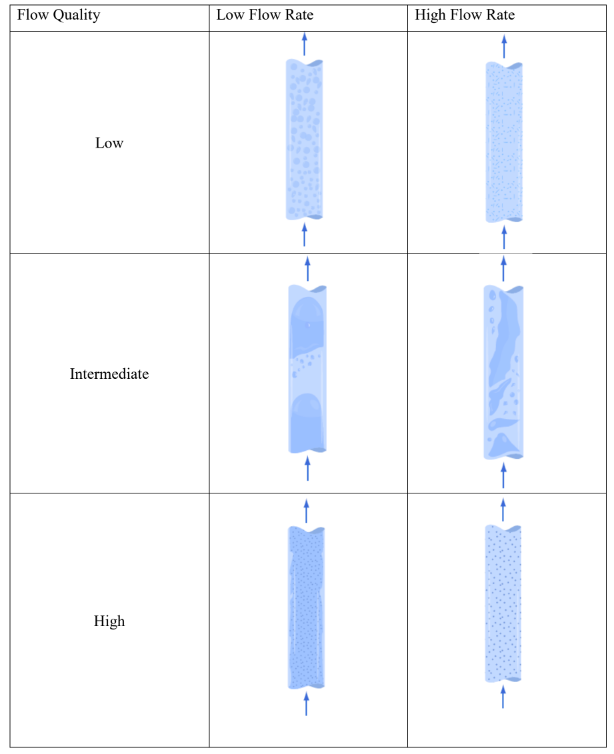
\includegraphics{flow-regime-map.png}
\caption{Flow Regime Map.}
\label{fig:flow-regime-map}
\end{figure}

\begin{marginfigure}
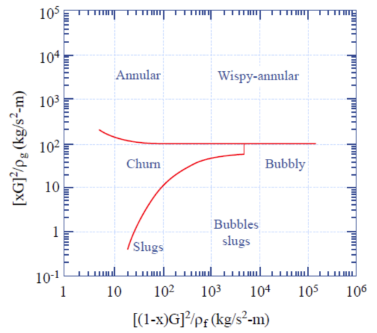
\includegraphics{flow-regime-map2.png}
\caption{Flow regime map for a two-phase flow system.}
\label{fig:flow-regime-map2}
\end{marginfigure}


For systems where complex two-phase flow behavior is expected, like a boiling water reactor, a flow regime map can be made as shown in Figure \ref{fig:flow-regime-map2} where an increase in the vertical axis is an increase in vapor mass flow rate; and an increase on the horizontal axis corresponds with increasing liquid mass flow rate.
\newthought{A wide range} of heat transfer phenomena occur in two-phase systems over the range of two-phase flow regimes.  These are illustrated graphically in Figure \ref{fig:two-phase-heat-xfer-regimes}.  

\begin{itemize}
\item Single-phase sub-cooled liquid enters at the bottom of the heated channel.  For sub-cooled liquids, equilibrium quality is negative.  

\item As the fluid approaches saturation temperature and $-0.25 < x_{eq} < 0$ vapor bubbles begin to form at nucleation sites along the wall; these bubbles are swept away from the wall and ultimately collapse.  This is referred to as \emph{sub-cooled nucleate boiling}.\marginnote{\textbf{Note:} the bubbles in sub-cooled nucleate boiling carry a great deal of energy with them.  This mode of heat transfer is both desirable and prevalent within pressurized water reactors.  The ability to predict the onset of this behavior and quantitatively model the improvement in heat transfer is one of the main incentives for discussing two-phase flow in this course.}

\item Note that sub-cooled nucleate boiling does not occur until \emph{after} the wall temperature has exceeded the fluid saturation temperature.  

\item As equilibrium quality increases above 0, void fraction increases and the two-phase flow regime begins to change also, transitioning from bubbly flow, to plug or slug flow depending on the mass flow rate.  Boiling water reactors can enter into this phase of two-phase heat transfer.

\item Mist flow begins at approximately $x_{eq} > 0.9$.

\end{itemize}

\begin{figure}
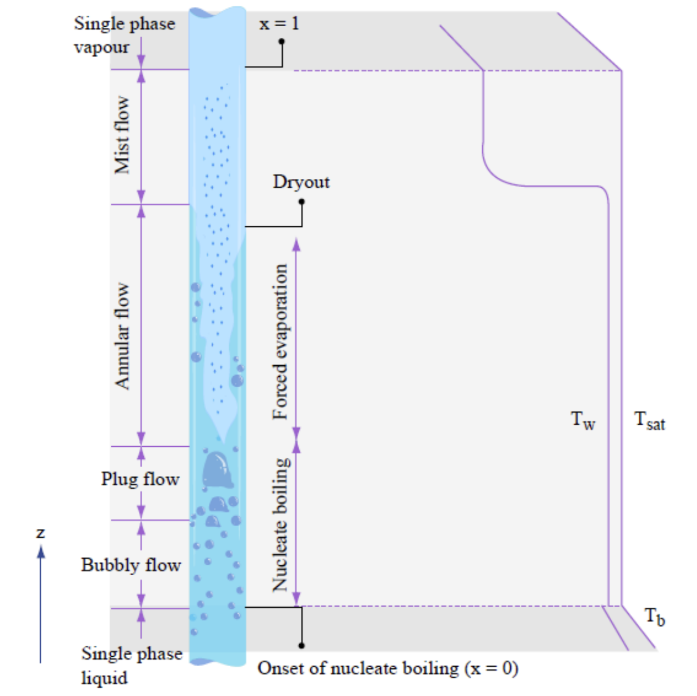
\includegraphics{two-phase-heat-xfer-regimes.png}
\caption{Two phase heat transfer regimes.}
\label{fig:two-phase-heat-xfer-regimes}
\end{figure}

\section{Applications for Nuclear Engineering}
Some relevant applications of two-phase flow and heat transfer in the engineering of nuclear reactors for power production are listed below.  This is by no means meant to be all-inclusive.

\begin{itemize}
\item \textbf{Boiling water reactor core.}  Two-phase flow exists for BWRs in normal operation.  Sub-cooled liquid ($x_{eq}<0$) enters the bottom of the reactor core.  The core exit condition is a saturated mixture with $x_{eq} \approx 12-15 \%$. 

\item \textbf{Steam generators for a PWR.}  Fluid conditions around the u-tubes for a recirculating SG of a PWR are similar to a BWR.  Sub-cooled liquid comes in and a saturated mixture of low quality is fed into the moisture separator and steam dryer apparatus.  

\item \textbf{PWR core.} Sub-cooled liquid enters a PWR; the high temperature water exiting a PWR core is also sub-cooled but its void fraction is positive.  As $x_{eq}$ approaches zero and as the fuel clad outer temperatures exceed local saturation temperature, nucleate boiling begins.  Nucleate boiling increases in intensity near the core exit.

\item \textbf{Reactor accident analysis.}  The transition from various regimes of two-phase heat transfer to critical heat flux is of great interest in the accident modeling community.  For PWRs the relevant mechanism is DNB; for BWRs the relevant mechanism is Dry-out.  These phenomena are a function of local heat flux as well as local hydraulic conditions.  If we can predict the heat flux at which CHF is likely $(q^{\prime \prime}_{\text{CHF}})$ then we can measure the ``Departure from Nucleate Boiling Ratio'' (DNBR) as $\sfrac{q^{\prime \prime}_{\text{CHF}}}{q^{\prime \prime}}$ which, to the extent we can estimate its value accurately, we always want to maintain above unity.

\item \textbf{NSSS Heat exchangers.}\marginnote{\textbf{NSSS} stands for \emph{nuclear steam supply system}.} Closed Feedwater Heaters, Reheaters, and Condensers are all elements of the nuclear steam supply system for a PWR based on the Rankine cycle and all involve extensive two-phase heat transfer phenomena.  

\item \textbf{PWR Pressurizer.} The pressurizer in a PWR during normal operations maintains a two-phase system of saturated liquid and saturated vapor in a low/no-flow configuration.  

\end{itemize}

